\documentclass[12pt,letterpaper]{article}

% Some packages:
\usepackage{listings}
\usepackage{graphicx}
\usepackage{color}

\begin{document}

\title{The Story Editor}
\author{Michael A. Gohde}
\date{February 24, 2017}
\maketitle

\section{Overview}
In order to make story authorship more accessible to a wider range of users, we have developed a graphical story editing and validation tool.
This tool should make it fairly straightforward to edit stories, convert between formats, run validation tasks, and submit drafts for publication.

This document will detail the Story Editor, its features, and its usage in a production environment.

\section{The Editor Window}

When it is first started, the Story Editor will create a blank story and display a window similar to what is depicted above. 
This window has a series of controls intended to allow a user to quickly engage in common tasks, such as adding new story nodes, setting the story title, and updating the contents of a given story node.

\begin{figure}
    \begin{center}
        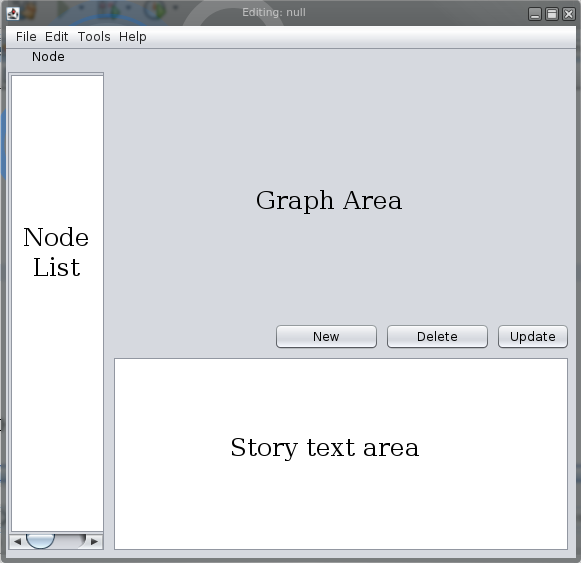
\includegraphics[scale=1]{emptywindow_with_labels.png}
    \end{center}
    \caption{Elements of the editor window}
\end{figure}

\begin{figure}
    \begin{center}
        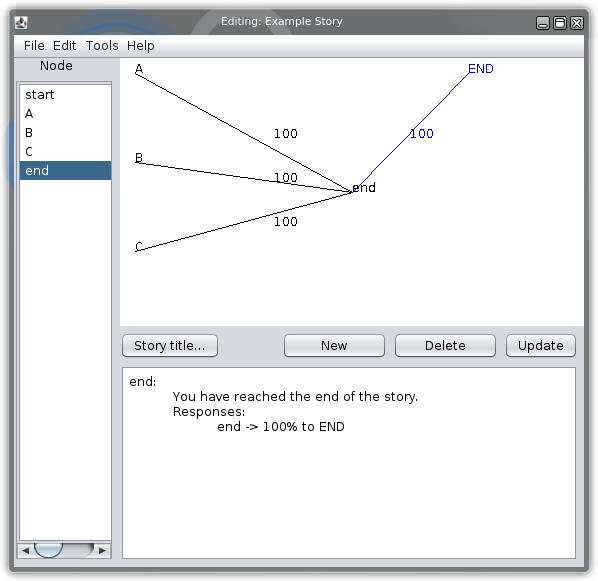
\includegraphics[scale=1]{examplewindow.png}
    \end{center}
    \caption{Editor window with active story}
\end{figure}

As shown above, the story editor window consists of the following major components:

\paragraph{Story text area}
The story text area displays the formatted text content within the selected story node. This field also allows the user to directly edit the ``source code'' of a story node.

\paragraph{Node List}
This pane contains a list of all nodes currently defined in the story. Each story node is effectively an individual story unit or decision point that is presented to the user.
The node list automatically updates when nodes are added to or removed from the story. 

\paragraph{Graph Area}
The Story Editor is capable of creating a graphical representation of the currently selected node and its relationships within the story.
When the Graph Area is filled, the set of all parent nodes is displayed on the right, the set of all child nodes is displayed on the left, and colored lines are drawn from the currently selected node to its parents and children.

\begin{center}
    \begin{tabular}{l|p{4in}}
    Color & Meaning\\ \hline \hline
    \textcolor{red}{Red} & The connected node does not exist.\\ \hline
    \textcolor{blue}{Blue} & The connected node is an endpoint for the story.\\ \hline
    Black & The connected node exists and is not an andpoint.\\ \hline
    \end{tabular}
    
    
    \textit{List of line colors and their meanings.}
\end{center}

\section{Menu Options}
Much of the validation, import, export, and settings functionality in the Story Editor is contained in its four menus.

\paragraph{The File Menu}
The File menu contains a set of items related to creating, importing, and exporting storylines.

\begin{center}
    \begin{tabular}{l|p{4in}}
    Item & Function\\ \hline \hline
    New & Creates a new storyline.\\ \hline
    Open... & Loads a file in the story definition format.\\ \hline
    Save... & Saves a file in the story definition format.\\ \hline
    Import from XML... & Loads a file in the XML story format used by the Nudge Support Toolset.\\ \hline
    Export from XML... & Saves a file in the XML story format.\\ \hline
    Import from Server... & Imports a storyline from a Nudge database server.\\ \hline
    Export to Server... & Exports a storyline to a set of temporary tables in a Nudge database server.\\ \hline
    Exit & Terminates the application.\\ \hline
    \end{tabular}
    \textit{List of items in the File menu and their functions.}
\end{center}

\paragraph{The Tools Menu}
The Tools menu contains a set of items related to changing global application settings, validating the current storyline, and collecting useful data.

\begin{center}
    \begin{tabular}{l|p{4in}}
    Item & Function\\ \hline \hline
    Sanity test & Runs a series of tests on the current storyline to determine if it is complete and sufficiently free of errors.\\ \hline
    Publish... & Exports the story to be installed in a production Nudge server.\\ \hline
    Set defaults... & Allows the user to specify various default values for save location, database server credentials, etc.\\ \hline
    Create account on database server... & Creates a user account so that stories can be imported from or saved to a nudge server for easy editing elsewhere.\\ \hline
    \end{tabular}
\end{center}

\section{Editing a story}
The story editing process is fairly straightforward. 

\section{Supported Story Formats}
In order to maintain wide compatibility with many external toolsets and applications, the Story Editor is capable of reading and writing stories in a large number of formats.
Among them, the story definitiion file, XML, and SQL formats provide the most utility with Nudge tools as implemented.

This section will provide examples of the same story exported to various formats.

\lstset{numbers=left, frame=shadowbox}
\begin{lstlisting}[breaklines=true, caption=Example story in story format.]
Title: Example Story
start:
        This is the first node in the story
        Responses:
                A -> 100% to A
                B -> 50% to B, 50% to C

A:
        You selected option choice A!
        Responses:
                Proceed -> 100% to end

B:
        You chose option B and were taken to node B.
        Responses:
                Proceed -> 100% to end

C:
        You chose option B but were taken to node C!
        Responses:
                Proceed -> 100% to end

end:
        You have reached the end of the story.
        Responses:
                end -> 100% to END
\end{lstlisting}

\begin{lstlisting}[breaklines=true, caption=Example story in XML format.]
<story title="Example Story">
        <node id="start">
                <text>This is the first node in the story</text>
                <answers>
                        <option>
                                <text>A</text>
                                <dest p="100">A</dest>
                        </option>
                        <option>
                                <text>B</text>
                                <dest p="50">B</dest>
                                <dest p="50">C</dest>
                        </option>
                </answers>
        </node>
        <node id="A">
                <text>You selected option choice A!</text>
                <answers>
                        <option>
                                <text>Proceed</text>
                                <dest p="100">end</dest>
                        </option>
                </answers>
        </node>
        <node id="B">
                <text>You chose option B and were taken to node B.</text>
                <answers>
                        <option>
                                <text>Proceed</text>
                                <dest p="100">end</dest>
                        </option>
                </answers>
        </node>
        <node id="C">
                <text>You chose option B but were taken to node C!</text>
                <answers>
                        <option>
                                <text>Proceed</text>
                                <dest p="100">end</dest>
                        </option>
                </answers>
        </node>
        <node id="end">
                <text>You have reached the end of the story.</text>
                <answers>
                        <option>
                                <text>end</text>
                                <dest p="100">END</dest>
                        </option>
                </answers>
        </node>
</story>
\end{lstlisting}

\begin{lstlisting}[breaklines=true, caption=Set of generated SQL statements.]
INSERT INTO tmpstorytable VALUES (1,'Example Story','start','This is the first node in the story',0);
INSERT INTO tmpanswers VALUES ('Example Story','start','A','A');
INSERT INTO tmpresults VALUES (1,'Example Story','start','A',0,100,'A');
INSERT INTO tmpanswers VALUES ('Example Story','start','B','B');
INSERT INTO tmpresults VALUES (2,'Example Story','start','B',0,50,'B');
INSERT INTO tmpresults VALUES (3,'Example Story','start','B',50,100,'C');
INSERT INTO tmpstorytable VALUES (2,'Example Story','A','You selected option choice A!',2);
INSERT INTO tmpanswers VALUES ('Example Story','A','A','Proceed');
INSERT INTO tmpresults VALUES (4,'Example Story','A','A',0,100,'end');
INSERT INTO tmpstorytable VALUES (3,'Example Story','B','You chose option B and were taken to node B.',2);
INSERT INTO tmpanswers VALUES ('Example Story','B','A','Proceed');
INSERT INTO tmpresults VALUES (5,'Example Story','B','A',0,100,'end');
INSERT INTO tmpstorytable VALUES (4,'Example Story','C','You chose option B but were taken to node C!',2);
INSERT INTO tmpanswers VALUES ('Example Story','C','A','Proceed');
INSERT INTO tmpresults VALUES (6,'Example Story','C','A',0,100,'end');
INSERT INTO tmpstorytable VALUES (5,'Example Story','end','You have reached the end of the story.',2);
INSERT INTO tmpanswers VALUES ('Example Story','end','A','end');
INSERT INTO tmpresults VALUES (7,'Example Story','end','A',0,100,'END');
\end{lstlisting}

\section{Remote story editing and storage}

One important possibility that the story editor enables is that of storing storylines on 
the a remote server so that can be more readily merged into Nudge's database. This approach
should also enable users to more easily manage and collaborate on their storylines from multiple
machines.

\subsection{Registering for a Collaborator ID}
In order to import or export storylines to a server, it is necessary to obtain two sets of credentials:
    
\begin{enumerate}
\item A database server login
\item A collaborator login
\end{enumerate}

The database server login allows a user to read and write from the Nudge database itself, while the collaborator login identifies storyline ownership and other key information.

In order to obtain a collaborator login, it is necessary to register with the database server. Registration is done
through the ``Create account on database server...'' item in the ``Tools'' menu. 

\begin{figure}
    \begin{center}
        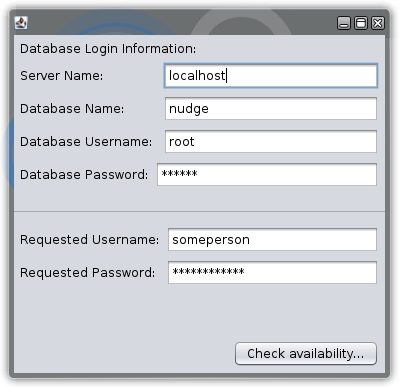
\includegraphics[scale=1]{registrationwindow.png}
    \end{center}
    \caption{Elements of the editor window}
\end{figure}

\begin{figure}
    \begin{center}
        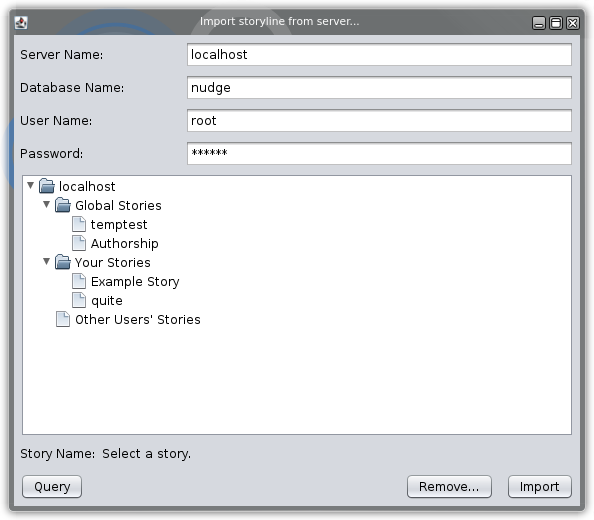
\includegraphics[scale=1]{importwindow.png}
    \end{center}
    \caption{Elements of the editor window}
\end{figure}

\section{Story merge support}

While not yet implemented, one important future direction for development is that of enabling
users to merge storylines together. While seemingly limited in usefulness, storyline merger
support will enable multiple users to collaboratively edit a sotryline. This, if used correctly, has
the potential to significantly reduce the time needed to write a storyline.

\end{document}